% Options for packages loaded elsewhere
% Options for packages loaded elsewhere
\PassOptionsToPackage{unicode}{hyperref}
\PassOptionsToPackage{hyphens}{url}
\PassOptionsToPackage{dvipsnames,svgnames,x11names}{xcolor}
%
\documentclass[
  letterpaper,
  DIV=11,
  numbers=noendperiod]{scrreprt}
\usepackage{xcolor}
\usepackage{amsmath,amssymb}
\setcounter{secnumdepth}{5}
\usepackage{iftex}
\ifPDFTeX
  \usepackage[T1]{fontenc}
  \usepackage[utf8]{inputenc}
  \usepackage{textcomp} % provide euro and other symbols
\else % if luatex or xetex
  \usepackage{unicode-math} % this also loads fontspec
  \defaultfontfeatures{Scale=MatchLowercase}
  \defaultfontfeatures[\rmfamily]{Ligatures=TeX,Scale=1}
\fi
\usepackage{lmodern}
\ifPDFTeX\else
  % xetex/luatex font selection
\fi
% Use upquote if available, for straight quotes in verbatim environments
\IfFileExists{upquote.sty}{\usepackage{upquote}}{}
\IfFileExists{microtype.sty}{% use microtype if available
  \usepackage[]{microtype}
  \UseMicrotypeSet[protrusion]{basicmath} % disable protrusion for tt fonts
}{}
\makeatletter
\@ifundefined{KOMAClassName}{% if non-KOMA class
  \IfFileExists{parskip.sty}{%
    \usepackage{parskip}
  }{% else
    \setlength{\parindent}{0pt}
    \setlength{\parskip}{6pt plus 2pt minus 1pt}}
}{% if KOMA class
  \KOMAoptions{parskip=half}}
\makeatother
% Make \paragraph and \subparagraph free-standing
\makeatletter
\ifx\paragraph\undefined\else
  \let\oldparagraph\paragraph
  \renewcommand{\paragraph}{
    \@ifstar
      \xxxParagraphStar
      \xxxParagraphNoStar
  }
  \newcommand{\xxxParagraphStar}[1]{\oldparagraph*{#1}\mbox{}}
  \newcommand{\xxxParagraphNoStar}[1]{\oldparagraph{#1}\mbox{}}
\fi
\ifx\subparagraph\undefined\else
  \let\oldsubparagraph\subparagraph
  \renewcommand{\subparagraph}{
    \@ifstar
      \xxxSubParagraphStar
      \xxxSubParagraphNoStar
  }
  \newcommand{\xxxSubParagraphStar}[1]{\oldsubparagraph*{#1}\mbox{}}
  \newcommand{\xxxSubParagraphNoStar}[1]{\oldsubparagraph{#1}\mbox{}}
\fi
\makeatother


\usepackage{longtable,booktabs,array}
\usepackage{calc} % for calculating minipage widths
% Correct order of tables after \paragraph or \subparagraph
\usepackage{etoolbox}
\makeatletter
\patchcmd\longtable{\par}{\if@noskipsec\mbox{}\fi\par}{}{}
\makeatother
% Allow footnotes in longtable head/foot
\IfFileExists{footnotehyper.sty}{\usepackage{footnotehyper}}{\usepackage{footnote}}
\makesavenoteenv{longtable}
\usepackage{graphicx}
\makeatletter
\newsavebox\pandoc@box
\newcommand*\pandocbounded[1]{% scales image to fit in text height/width
  \sbox\pandoc@box{#1}%
  \Gscale@div\@tempa{\textheight}{\dimexpr\ht\pandoc@box+\dp\pandoc@box\relax}%
  \Gscale@div\@tempb{\linewidth}{\wd\pandoc@box}%
  \ifdim\@tempb\p@<\@tempa\p@\let\@tempa\@tempb\fi% select the smaller of both
  \ifdim\@tempa\p@<\p@\scalebox{\@tempa}{\usebox\pandoc@box}%
  \else\usebox{\pandoc@box}%
  \fi%
}
% Set default figure placement to htbp
\def\fps@figure{htbp}
\makeatother





\setlength{\emergencystretch}{3em} % prevent overfull lines

\providecommand{\tightlist}{%
  \setlength{\itemsep}{0pt}\setlength{\parskip}{0pt}}



 


\KOMAoption{captions}{tableheading}
\makeatletter
\@ifpackageloaded{bookmark}{}{\usepackage{bookmark}}
\makeatother
\makeatletter
\@ifpackageloaded{caption}{}{\usepackage{caption}}
\AtBeginDocument{%
\ifdefined\contentsname
  \renewcommand*\contentsname{Table of contents}
\else
  \newcommand\contentsname{Table of contents}
\fi
\ifdefined\listfigurename
  \renewcommand*\listfigurename{List of Figures}
\else
  \newcommand\listfigurename{List of Figures}
\fi
\ifdefined\listtablename
  \renewcommand*\listtablename{List of Tables}
\else
  \newcommand\listtablename{List of Tables}
\fi
\ifdefined\figurename
  \renewcommand*\figurename{Figure}
\else
  \newcommand\figurename{Figure}
\fi
\ifdefined\tablename
  \renewcommand*\tablename{Table}
\else
  \newcommand\tablename{Table}
\fi
}
\@ifpackageloaded{float}{}{\usepackage{float}}
\floatstyle{ruled}
\@ifundefined{c@chapter}{\newfloat{codelisting}{h}{lop}}{\newfloat{codelisting}{h}{lop}[chapter]}
\floatname{codelisting}{Listing}
\newcommand*\listoflistings{\listof{codelisting}{List of Listings}}
\makeatother
\makeatletter
\makeatother
\makeatletter
\@ifpackageloaded{caption}{}{\usepackage{caption}}
\@ifpackageloaded{subcaption}{}{\usepackage{subcaption}}
\makeatother
\usepackage{bookmark}
\IfFileExists{xurl.sty}{\usepackage{xurl}}{} % add URL line breaks if available
\urlstyle{same}
\hypersetup{
  pdftitle={Armein Z. R. Langi},
  pdfauthor={131902360 Armein Z R Langi},
  colorlinks=true,
  linkcolor={blue},
  filecolor={Maroon},
  citecolor={Blue},
  urlcolor={Blue},
  pdfcreator={LaTeX via pandoc}}


\title{Armein Z. R. Langi}
\usepackage{etoolbox}
\makeatletter
\providecommand{\subtitle}[1]{% add subtitle to \maketitle
  \apptocmd{\@title}{\par {\large #1 \par}}{}{}
}
\makeatother
\subtitle{Portfolio Asesmen II-2100 KIPP}
\author{131902360 Armein Z R Langi}
\date{2025-09-15}
\begin{document}
\maketitle

\renewcommand*\contentsname{Table of contents}
{
\hypersetup{linkcolor=}
\setcounter{tocdepth}{2}
\tableofcontents
}

\bookmarksetup{startatroot}

\chapter*{Selamat Berjumpa}\label{selamat-berjumpa}
\addcontentsline{toc}{chapter}{Selamat Berjumpa}

\markboth{Selamat Berjumpa}{Selamat Berjumpa}

\begin{figure}[H]

{\centering 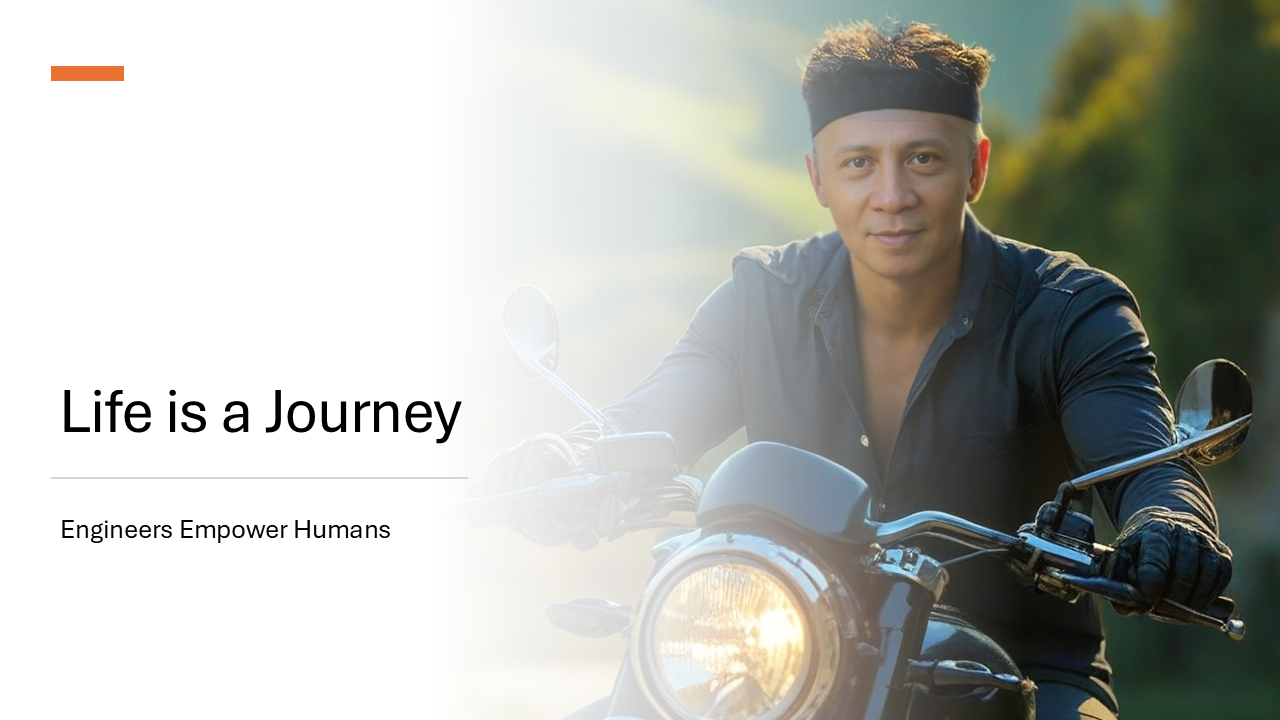
\includegraphics[width=9.5\linewidth,height=\textheight,keepaspectratio]{images/AZRL.png}

}

\caption{About Me}

\end{figure}%

Armein Z R Langi adalah Guru Besar di Sekolah Teknik Elektro dan
Informatika ITB, dosen ITB sejak Desember 1987, mantan Rektor
Universitas Kristen Maranatha, 1 Maret 2016 s/d 29 Februari 2020, mantan
Kepala Pusat Penelitian Teknologi Informasi dan Komunikasi (PP-TIK) ITB
November 2005 s/d Maret 2010, dan Sekretaris MWA ITB Mei 2010-Jan 2011.

Lahir di Tomohon 1962 dari pasangan Manado dan Sunda. Saat ini tinggal
di Bandung, menikah dengan Ina dan dikaruniai empat anak. Ayah dari
Gladys, Kezia, Andria, dan Marco.

Sharing pikiran singkat ada di blog \url{https://azrl.wordpress.com}.
Facebookk: armein\_langi

Andria, putri saya, lumayan sering membaca blog ini. Dia juga sumber
inspirasi tulisan saya. Dia senang menceritakan jokes pada saya, dan
kalau bagus saya tulis di sini, terutama seri Kocak Ala Andria. Dan dia
suka heran, karena isinya sudah berbeda. Memang saya senang
mengubah-ngubah cerita karena saya tidak suka menjiplak mentah-mentah.
Minggu lalu tidak sengaja dia memuji tulisan blog ini.

``Papa\ldots{} papa\ldots{} ``, tanyanya, ``Tulisan blog papa itu
copy-paste dari tulisan orang ya\ldots?''

Haa? Ya nggak mungkin lah. Kecuali lirik lagu, semua artikel di sini
ditulis sendiri.

``Ah bohong, soalnya tulisannya terlalu banyak\ldots.'' katanya tetap
tidak percaya, ``Nggak mungkinlah papa tulis sendiri\ldots{}''

Hehe, saya tersenyum sambil membelai Andria, karena buat saya itu adalah
ultimate compliment. Thanks sweetheart\ldots{}

Jadi kalau orang tidak percaya bahwa sesuatu itu karya anda, anda yang
buat, jangan marah. Itu adalah pujian yang sejati.

\bookmarksetup{startatroot}

\chapter{UTS-1 All About Me}\label{uts-1-all-about-me}

Aku Ivant Samuel Silaban. Seorang mahasiswa Teknik Informatika di
Institut Teknologi Bandung, dan ini adalah tahun ketigaku. Aku anak
laki-laki satu-satunya dari empat bersaudara, sebuah posisi yang
menanamkan ekspektasi untuk menjadi pemimpin dan pelindung di masa
depan. Aku lahir di Balige, kota sunyi di tepi Danau Toba, sebelum
akhirnya menjadikan Bandung rumah baru untuk menempa ilmu.

Secara alamiah, aku adalah seorang INTP. Artinya, aku punya dua sifat
bawaan:

\begin{enumerate}
\def\labelenumi{\arabic{enumi}.}
\item
  Aku suka mengeksplor banyak hal (sisi `P' - Prospecting), yang
  menjelaskan kenapa aku ``gampang bosan'' dan hobiku adalah ``mencoba
  hal baru''.
\item
  Aku suka berdebat (sisi `T' - Thinking). Aku suka menganalisis,
  mencari kebenaran logis, dan menantang ide yang tidak efisien.
\end{enumerate}

Ironisnya, aku dididik untuk jadi bijaksana (kata Ayah) dan mengutamakan
perasaan orang lain (kata Ibu). Kombinasi ini menghasilkan produk
menarik: seorang INTP (logis \& suka berdebat) yang terjebak dalam peran
`people-pleaser' (harmonis \& pasif). Aku jadi manusia yang mandiri
(anak asrama), tapi sangat bergantung pada validasi eksternal.

Hobi? Aku nggak punya satu hobi pasti. Aku gampang bosan, jadi hobiku
adalah mencoba hal baru. Mungkin itu hobi yang sebenarnya: eksplorasi.
Aku juga suka mengamati interaksi manusia, mencari keindahan di
momen-momen kecil yang sering terlewat. Aku adalah pengamat interaksi
manusia. Aku suka mencari keindahan di momen kecil. Tapi aku juga punya
`bug' besar: aku lebih mengutamakan kenyamanan orang lain daripada
kenyamananku sendiri.

\section{\texorpdfstring{\textbf{Tirani Harmoni: Saat `Baik' Menjadi
Bumerang}}{Tirani Harmoni: Saat `Baik' Menjadi Bumerang}}\label{tirani-harmoni-saat-baik-menjadi-bumerang}

Aku dibesarkan untuk jadi `anak baik'. Masalahnya, `baik' sering
disalahartikan sebagai `pasif'. Aku terjebak dalam Kepasifan (Passivity,
di mana aku membiarkan orang lain menulis dialog di cerita hidupku. Aku
jadi pahlawan di cerita mereka, tapi jadi korban di ceritaku sendiri.

Ini adalah Cerita Kontaminasi (Contamination Story) yang klasik. Niat
baikku (`positif') diracuni oleh kepasifanku, yang membuatku
dimanfaatkan oleh mereka (`negatif'). Aku membiarkan `tumpahan minyak'
ini meracuni kesehatan mentalku.

\emph{Tragedi `Solo Tubes'}

Dari tahun pertama, setiap ada tugas berkelompok, kemungkinan besar ada
paling tidak satu orang di kelompokku yang menjadi `beban' kelompok.
Tetapi selama tahun pertama, aku beruntung masih punya satu orang yang
menjadi `sepuh' kelompok, jadi aku tidak terlalu capek untuk
berkontribusi mengerjakan tubes-tubes. Namun, semua berganti saat tubes
kedua mata kuliah aljabar linear dan geometri, dimana di H-1, ada teman
sekelompokku yang masih selesai bagian desain figmanya doang, sedangkan
aku dan temanku yang satu lagi sudah kelar backend dari minggu pertama
tugas tersebut diturunkan. Padahal selama tiga minggu lamanya, kami
bertanya apakah sudah aman atau belum, dan dia selalu menjawab aman. Ini
membuatku di hari-h deadline mengerjakan website sendirian sampai aku
harus bolos kelas seharian. Kuharap ini adalah pertama dan terakhir
kalinya aku mendapatkan kelompok seperti ini. Dan apakah ini memang
sudah berakhir? Oh belum. Aku justru mendapatkan sesuatu yang bahkan
jauh lebih parah. Di semester 4, ada satu week yang diisi ama 3 deadline
tubes, yaitu tubes Sistem Operasi, Basis Data, dan Jaringan Komputer.\\
Untuk Sistem Operasi, terdiri dari lima milestone dengan soft deadline.
Dimana milestone 1 dikerjakan oleh dua orang teman saya, lalu aku
melakukan finishing pada milestone 1 dan sekalian mengerjakan sampai
selesai milestone 2. Lalu pada milestone 2, temanku hanya mengerjakan
setengah dan aku melanjutkannya. Dan ternyata bagian yang harus aku
lanjutkan adalah salah satu bagian tersulit di tugas ini. Dan akhirnya
selesai di h-7 deadline.\\
Tidak cukup sampai situ, selama dua atau tiga hari, aku membawa laptopku
servis karena rawan blue screen, sehingga aku meminta temanku untuk
melanjutkan milestone selanjutnya. Saat itu, aku mengantar laptopku
bersama teman satu kos yang merupakan teman satu kelompokku juga. Selama
tiga hari aku menunggu sambil mengerjakan tugas lain yang bisa
dikerjakan lewat HP, dan akhirnya selesai. Paling menyedihkannya,
ternyata tidak ada progress signifikan dari teman kelompokku, bahkan
teman satu kosku selama ini terlalu asik bermain game. Jujur, aku sangat
kesal ke teman satu kos ini apalagi ketika dia mengakui dia gak paham
dengan tugas ini, tetapi aku selalu menahan diriku untuk tidak marah,
dan mengambil keputusan untuk tidak tidur selama beberapa hari kedepan
untuk menyelesaikan tugas ini. Tugas ini akhirnya dikumpul apa adanya,
masih banyak masalah karena kecerobohanku selama mengerjakan tugas
ini.\\
Dua hari kemudian adalah deadline tugas besar basis data. Tugas ini
punya tiga milestone, dan selama tiga milestone ini, tidak semua
kelompokku aktif, dan aku tidak terlalu mempermasalahkannya karena
akhirnya selesai juga. Dan dua hari setelahnya adalah deadline tugas
besar jaringan komputer. Tugas ini punya dua bagian besar, dan jauh
sebelum deadline, aku sudah menyelesaikan satu bagian yang dimana
berarti aku sudah kontribusi 40-50\%. Untuk bagian 2, aku sudah bikin
kode awalnya, tinggal tiga teman kelompokku menyesuaikan. Dan ya,
ternyata tidak ada progres signifikan dan aku terpaksa solo tugas ini
lagi, dan ironisnya, aku sekelompok dengan teman satu kosku itu.\\
Dan yang paling aneh dari semuanya adalah teman satu kosku itu. Dia
bahkan tidak mengucapkan `Maaf' atau `Terima Kasih' sama sekali. Dan
yang paling mengecewakan dari dia adalah dia masih selalu
meninggalkanku, bahkan di saat aku lagi kurang enak badan karena
beberapa hari tidak tidur dan persiapan untuk uas yang terlalu
memaksakan diriku. Aku akhirnya menyadari bahwa aku baru saja
mengorbankan kewarasanku untuk `harmoni' palsu. Ini adalah ``daya tarik
interpersonal'' yang sangat error. Ternyata `daya tarik
interpersonal'-ku adalah semacam magnet bagi freeloader profesional
(just kidding :D).

\subsection{\texorpdfstring{\textbf{Kontaminasi dari Orang
Lain}}{Kontaminasi dari Orang Lain}}\label{kontaminasi-dari-orang-lain}

Aku punya teman-teman yang, jujur saja, nggak punya arah. Aku membantu
mereka, membagikan hal positif, dan nggak pernah meninggalkan mereka.
Aku berharap `kebaikan'-ku akan mengubah mereka. Hasilnya? Mereka
mengecewakanku berkali-kali. Aku jadi si `cuek' di luar, tapi `kesal' di
dalam.

\section{\texorpdfstring{\textbf{Menulis Ulang Manual:
Penebusan}}{Menulis Ulang Manual: Penebusan}}\label{menulis-ulang-manual-penebusan}

Setiap malam aku berpikir: apa mereka yang `aneh'? Atau aku yang terlalu
naif?

`Benturan'-nya bersifat batin. Momen `terbentuk'-nya datang saat aku
menemukan jawaban di Kitab Amsal: ``Siapa bergaul dengan orang bijak
menjadi bijak, tetapi siapa berteman dengan orang bebal menjadi
malang.''

Ayat ini bukan sekadar nasihat. Bagiku, ini adalah `momen berkilau'
(sparkling moment), momen `penalaran otobiografis' yang menyadarkanku.
Aku sadar bahwa `bijaksana' seperti kata Ayahku, bukan berarti `pasif'.
Bijaksana berarti punya Agensi (Agency) untuk memilih siapa yang layak
ada di hidup kita.

Aku pun mengambil keputusan. Aku `terpaksa' meninggalkan mereka. Awalnya
sakit, tapi ini jalan yang harus aku tempuh.

Jadi, siapa aku? Aku Ivant. Aku masih `anak baik' dan `pengamat
manusia'. Tapi manual operasiku sudah diperbarui. `Baik' versiku
sekarang juga berarti `baik' ke diriku sendiri. Dan `daya tarik
interpersonal'-ku yang baru adalah otentisitas, bukan lagi kepasifan
yang `nggak enakan'.

\bookmarksetup{startatroot}

\chapter{UTS-2 My Songs for You}\label{uts-2-my-songs-for-you}

\section{Lyrics}\label{lyrics}

Don't Stop Me Now Lirik by Freddie Mercury Music: Queen

\begin{figure}[H]

{\centering 
\includegraphics[width=9.5\linewidth,height=\textheight,keepaspectratio]{My_Song_for_You/../images/photo1.jpeg}

}

\caption{Queen}

\end{figure}%

{[}Intro{]} Tonight, I'm gonna have myself a real good time I feel alive
And the world, I'll turn it inside out, yeah I'm floatin' around in
ecstasy So don't stop me now Don't stop me `Cause I'm havin' a good time
Havin' a good time

{[}Verse 1{]} I'm a shootin' star, leapin' through the sky like a tiger
Defyin' the laws of gravity I'm a racin' car, passin' by like Lady
Godiva I'm gonna go, go, go, there's no stoppin' me

{[}Pre-Chorus{]} I'm burnin' through the sky, yeah Two hundred degrees,
that's why they call me Mister Fahrenheit I'm travelling at the speed of
light I wanna make a supersonic man outta you

{[}Chorus{]} Don't stop me now I'm havin' such a good time, I'm havin' a
ball Don't stop me now If you wanna have a good time, just give me a
call (Don't stop me now) `Cause I'm havin' a good time (Don't stop me
now) Yes, I'm havin' a good time I don't wanna stop at all, yeah

{[}Verse 2{]} I'm a rocket ship on my way to Mars on a collision course
I am a satellite, I'm out of control I'm a sex machine, ready to reload
like an atom bomb About to oh, oh, oh, oh, oh, explode

{[}Pre-Chorus{]} I'm burnin' through the sky, yeah Two hundred degrees,
that's why they call me Mister Fahrenheit I'm travellin' at the speed of
light I wanna make a supersonic woman of you

{[}Bridge{]} (Don't stop me, don't stop me, don't stop me) Hey, hey, hey
(Don't stop me, don't stop me, ooh, ooh, ooh) I like it (Don't stop me,
don't stop me, hey, alright) Have a good time, good time (Don't stop me,
don't stop me) Woah Let loose, honey, alright

{[}Guitar Solo{]}

{[}Pre-Chorus{]} Oh, I'm burnin' through the sky, yeah Two hundred
degrees, that's why they call me Mister Fahrenheit, hey Travellin' at
the speed of light I wanna make a supersonic man outta you, hey, hey
{[}Chorus{]} Don't stop me now I'm havin' such a good time, I'm havin' a
ball Don't stop me now (Ooh) If you wanna have a good time (Alright),
just give me a call (Don't stop me now) `Cause I'm havin' a good time
(Hey, hey) (Don't stop me now) Yes, I'm havin' a good time I don't wanna
stop at all

{[}Outro{]} Ah, da, da, da, da Da, da, ah, ah Ah, da, da, ah, ah, ah Ah,
da, da Ah, da, da, ah, ah Ooh, ooh-ooh, ooh-ooh

\section{Makna}\label{makna}

Orang lain mungkin tahu aku sebagai INTP yang ``malas'' dan ``gampang
bosan'', atau si ``nggak enakan'' yang pasif. Aku adalah orang yang
paling jago nge-stop diriku sendiri.

Tapi sejak ada kamu\ldots{}

Kamu adalah `benturan' yang membuatku `terbentuk'. Kamu adalah `Agensi'
yang membuatku berani jadi logis sekaligus peduli. Kamu adalah alasan
kenapa, untuk pertama kalinya, aku bisa mendengarkan lagu ini dan merasa
jujur.

Aku bukan Freddie Mercury. Aku bukan `Mister Fahrenheit'.

Tapi karena kamu, aku merasa alive. Dan aku finally bisa bilang ke
diriku sendiri\ldots{}

\ldots Don't stop me now.

\bookmarksetup{startatroot}

\chapter{UTS-3 My Stories for You}\label{uts-3-my-stories-for-you}

\emph{(Narasi Penemuan Diri)}

Ini bukan cerita tentang bakat alami. Aku tidak punya itu.

Ini adalah cerita tentang ``penemuan diri'' yang brutal. Tentang siklus.
Tentang jatuh, hancur, lalu bangkit lagi. Ini adalah kisah inspiratif
yang ingin aku bagikan: kisah tentang resiliensi.

\section{\texorpdfstring{\textbf{Bab 1: Agensi Melawan
Siklus}}{Bab 1: Agensi Melawan Siklus}}\label{bab-1-agensi-melawan-siklus}

Aku nggak merasa punya talenta bawaan apa-apa. Waktu kecil, aku melihat
teman-temanku jago di banyak hal. Aku? Aku merasa biasa saja. Ini bisa
jadi Cerita Kontaminasi (Contamination Story) awalku: narasi tentang
anak yang terlahir `biasa saja'.

Tapi aku menolak narasi itu. Aku percaya pada Agensi (Agency), bahwa aku
adalah aktor utama dalam ceritaku.

`Momen berkilau' pertamaku datang dari buku ensiklopedia tebal saat
kelas 4 SD. Itu memicu rasa ingin tahu. Puncaknya di kelas 5, aku yang
merasa paling kurang di matematika, nekat ikut seleksi tim olimpiade dan
lolos (dengan cara yang agak ajaib dan penuh tebakan).

Kejadian itu menjadi katalis. Aku mulai fokus. Yang dulu paling lama
pulang sekolah, akhirnya bisa jadi juara kelas.

Tapi, ceritaku bukanlah garis lurus. Ia sebuah siklus yang berulang:
Kontaminasi -\textgreater{} Penebusan -\textgreater{} Kontaminasi
-\textgreater{} Penebusan.

Polanya selalu sama: aku menjadi malas, sombong, dan terlena. Ini
`Kontaminasi'-ku.

\begin{itemize}
\tightlist
\item
  Siklus \#1 (SMP): Aku lolos kelas unggulan, lalu terlena. Aku jadi
  pemalas, tidak belajar. Aku masuk `zona kuning' zona waspada keluar
  dari kelas unggul. Teman-temanku mulai meninggalkanku. Itu `benturan'
  pertamaku. Aku down.\\
  Tidak ada yang bisa mempercayaiku. Teman-temanku selalu menghindariku
  jika ada tugas kelompok, bermain, dan kegiatan-kegiatan lain. Bahkan
  aku pernah merasa bahwa aku sedang di-bully mereka (tetapi ini
  sebenarnya karena efek overthinking).
\end{itemize}

Tapi `benturan' itu juga yang membuatku `terbentuk'. Di kelas 9, aku
paksa diriku fokus. Hasilnya? Aku lolos ke SMA Unggulan, mengalahkan
temanku yang dulu selalu juara kelas. Itu Penebusan pertamaku. Bahkan,
selama kelas 9, aku berhasil membuat mereka menganggap aku sebagai
seorang teman. Jadi aku akhirnya selalu diajak untuk bermain sama,
belajar sama, dan akhirnya aku bisa eksplorasi lebih jauh. Bahkan mereka
kadang minta bantuan akademik dari aku.

\begin{itemize}
\tightlist
\item
  Siklus \#2 (SMA): Pola itu kembali, dan lebih parah. Efek daring
  karena COVID-19, aku hancur oleh games. Emosiku tidak stabil,
  akademikku hancur lebur. `Kontaminasi' kali ini terasa fatal. Semua
  berawal dari selama libur yang aku kebanyakan begadang untuk bermain
  games dan menonton anime. Lalu saat sudah mulai SMA, aku mengganggap
  remeh materi-materi SMA, berpikir sama seperti waktu SMP yang dimana
  aku tidak pernah belajar masih bisa mendapatkan nilai tinggi. Bahkan
  aku yang biasanya semangat ikut olimpiade, kali ini sirna. Aku terlalu
  sering bermain games dan hiburan lainnya. Akhirnya aku tertampar
  nilai-nilaiku yang hancur, dan aku sadar bahwa SMA ini adalah bukan
  SMA biasa. Soal-soal di SMA ini udah sangat jauh lebih sulit dari yang
  aku bayangkan. `Benturan' kedua datang saat kami kembali ke asrama.
  Aku sadar betapa hancurnya diriku. Dan sekali lagi, `benturan' itu
  memaksaku `terbentuk' kembali. Setelah kegiatan pra-asrama di SMA-ku
  (Orientasi), aku merasa kalau aku punya fisik yang sangat buruk, pola
  pikir yang kacau. Nilai-nilaiku pun tetap sama hancurnya, bahkan kali
  ini aku hampir tinggal kelas karena satu mata pelajaran yang di bawah
  rata-rata.\\
  Akhirnya aku berpikir untuk berubah. Langkah awal yang aku ambil
  adalah membatasi diriku secara ketat terkait konten media sosial dan
  games yang aku mainin. Lalu waktu yang biasanya aku gunakan untuk
  bermain game, aku convert ke berolahraga. Ini adalah tahap awal
  perubahanku. Selama libur menuju kelas 12, aku selalu berolahraga,
  bahkan setelah masuk asrama kembali, aku tetap berolahraga. Aku yang
  biasanya tidur di kelas (efek begadang saat libur), bisa tetap bangun.
  Dan motivasi akademikku seketika naik setelah aku mendapatkan nilai
  yang sangat tinggi di mata pelajaran yang selama kelas 10 dan 11
  selalu remedial.
\end{itemize}

\section{\texorpdfstring{\textbf{Bab 2: Penemuan
Diri}}{Bab 2: Penemuan Diri}}\label{bab-2-penemuan-diri}

Pola ini---jatuh karena kemalasan, lalu bangkit karena `tamparan'
realita---adalah inti ``penemuan diriku''.

``Keautentikan''-ku ada di sini: Aku bukan orang yang konsisten rajin.
Aku adalah orang yang selalu bisa bangkit lagi.

``Inspirasi'' yang ingin aku bagikan adalah ini: Lolos ke ITB bukanlah
hasil dari bakat alami atau konsistensi tanpa cela. Itu adalah hasil
dari Penebusan yang terjadi selama ini.

Narasi negatif ``aku tidak punya talenta'' pada akhirnya diubah menjadi
narasi positif ``aku adalah bukti bahwa resiliensi dan kerja keras
mengalahkan bakat''. Agensiku bukanlah konsistensi, tapi resiliensi. Dan
itu, kurasa, adalah cerita yang layak dibagikan.

\bookmarksetup{startatroot}

\chapter{\texorpdfstring{Sumber
\href{StrengthsProfile-Armein-Langi.pdf}{VIA
assessment}}{Sumber VIA assessment}}\label{sumber-via-assessment}

\bookmarksetup{startatroot}

\chapter{UTS-4: My SHAPE}\label{uts-4-my-shape}

\textbf{Nama:} Ivant Samuel Silaban

\section{S - Signature Strengths (Kekuatan
Khas)}\label{s---signature-strengths-kekuatan-khas}

\begin{enumerate}
\def\labelenumi{\arabic{enumi}.}
\item
  \textbf{Kegigihan (Persistence) \& Resiliensi:} Kekuatan inti dari
  cerita dari my stories for you. Terbukti dari ``Siklus Terbentur,
  Terbentuk''. Aku mungkin jatuh ke dalam kemalasan atau down
  (Kontaminasi), tapi aku selalu bangkit kembali (Penebusan).
\item
  \textbf{Kebaikan Hati (Kindness) \& Empati:} Kekuatan inti dari cerita
  all about me. Ini adalah akar dari ``Tirani Harmoni''. Meskipun sempat
  menjadi `bug', ini tetap kekuatan fundamentalku. Aku ``mengutamakan
  perasaan orang lain'' dan ``peduli''.
\item
  \textbf{Kecerdasan Sosial \& Perspektif:} Dari all about me. Aku
  adalah ``pengamat interaksi manusia'' dan ``suka mencari keindahan di
  momen kecil''. Ini adalah kekuatan analitis di ranah sosial.
\item
  \textbf{Rasa Ingin Tahu (Curiosity) \& Cinta Belajar:} Dari cerita my
  stories for you. Terbukti dari momen `Ensiklopedia' dan hobi
  ``eksplorasi'' di cerita all about me.
\end{enumerate}

\section{H - Heart (Hati: Nilai Inti \&
Gairah)}\label{h---heart-hati-nilai-inti-gairah}

Berdasarkan Latihan Klarifikasi Nilai:

\textbf{Nilai Inti \#1: Pertumbuhan Pribadi:} Aku sangat menghargai
proses `terbentuk' setelah `terbentur'. Aku percaya pada perbaikan diri
yang terus-menerus.

\textbf{Nilai Inti \#2: Kebijaksanaan (Wisdom):} Didikan Ayah dan
pelajaran dari Amsal (all about me). Aku menghargai pengambilan
keputusan yang tepat dan berani (seperti menetapkan boundaries).

\textbf{Nilai Inti \#3: Harmoni \& Koneksi:} Didikan Ibu (all about me).
Meski ``Tirani Harmoni'' itu buruk, Harmoni yang sehat tetap jadi nilai
inti buat aku.

\textbf{Aku Bersemangat Tentang:} Memecahkan pola yang rumit (baik di
dalam kode maupun dalam interaksi manusia) dan membantu orang lain
menemukan `benturan' mereka agar bisa `terbentuk'.

\section{A - Aptitudes \& Acquired Skills (Bakat \&
Keterampilan)}\label{a---aptitudes-acquired-skills-bakat-keterampilan}

\textbf{Inventaris pribadi:}

\subsection{Hard Skills (Teknis):}\label{hard-skills-teknis}

\begin{itemize}
\tightlist
\item
  \textbf{Pemrograman:} Bahasa pemrograman, algoritma, struktur data.
\item
  \textbf{Analisis Data dan Riset (SQL, Statistik):} Analisis pola dan
  menyusun model
\item
  \textbf{Matematika dan Logika:} Kemampuan berpikir deduktif dan
  abstrak
\item
  \textbf{Desain Konseptual / Eksperimen teoretis:} Simulasi, modeling,
  dan framework, algoritma, dan model baru
\end{itemize}

\subsection{Soft Skills (Non-Teknis):}\label{soft-skills-non-teknis}

\textbf{Kesadaran Diri (Self-Awareness):} Aku sangat sadar akan pola
siklus (malas-bangkit) dan kelemahanku (`nggak enakan').

\textbf{Manajemen Krisis (di bawah tekanan):} Terbukti dari ``Tragedi
Solo Tubes'' dari cerita all about me. Aku bisa mengerjakan 3 deadline
besar sendirian (meski dengan konsekuensi).

\textbf{Empati \& Mendengarkan Aktif:} Kemampuan memahami kebutuhan
orang lain dari cerita all about me

\textbf{Resiliensi:} Kemampuan untuk bangkit dari kegagalan
akademik/pribadi.

\section{P - Personality (Profil
Kepribadian)}\label{p---personality-profil-kepribadian}

Berdasarkan tes 16Personalities:

\textbf{Tipe MBTI:} INTP

\textbf{Analisis (Mengapa ini cocok):} Profil ini adalah pusat dari
konflik narasiku.

\begin{itemize}
\item
  \textbf{(I) Introvert \& (N) Intuitive:} Ini adalah mode ``Pengamat''.
\item
  \textbf{(T) Thinking vs.~(F) Feeling:} Ini adalah inti ``Tirani
  Harmoni'' (UTS-1). Secara alamiah, aku suka berdebat (T), tapi didikan
  memaksa aku bertindak sebagai F (Harmoni). ``Penebusan'' (Amsal)
  adalah momen T (Thinking) aku mengambil alih `Agensi'.
\item
  \textbf{(P) Perceiving vs.~(J) Judging:} Ini adalah inti ``Siklus
  Terbentur''. Mode default aku adalah P (suka mengeksplor, gampang
  bosan, malas). Mode ``terbentuk'' aku adalah J (bangkit, grinding
  UAS). Kecenderungan ``mendekati INTJ'' adalah `Agensi'-ku saat
  diaktifkan oleh `benturan'.
\end{itemize}

\textbf{Gaya Kerja yang Disukai:} Lingkungan yang logis dan adil. Aku
butuh kebebasan untuk \textbf{mengeksplor (P)}, tapi juga
\textbf{deadline yang jelas (J)} untuk memicu performa puncak.

\section{E - Experiences (Pengalaman
Hidup)}\label{e---experiences-pengalaman-hidup}

Pelajaran Kunci dari Identitas Naratif:

\textbf{Peristiwa:} ``Siklus Terbentur, Terbentuk'' (SMP \& SMA).

\textbf{Pelajaran:} Kegagalan adalah `benturan' yang diperlukan untuk
`terbentuk'. Resiliensi lebih penting daripada kesempurnaan.

\textbf{Peristiwa:} ``Tirani Harmoni'' \& Konflik Teman.

\textbf{Pelajaran:} Menjadi `baik' (nilai H) bukan berarti menjadi
`pasif' (kelemahan). Kebijaksanaan (nilai H) berarti memiliki `Agensi'
untuk menetapkan batasan yang sehat.

\textbf{Peristiwa:} ``Olimpiade Matematika `Ajaib'\,''.

\textbf{Pelajaran:} `Agensi' (keberanian mencoba) dapat menciptakan
`bakat' yang tidak ada sebelumnya.

\section{Piagam Pribadi}\label{piagam-pribadi}

\textbf{Pernyataan Misi Pribadi:}: ``Menggunakan kekuatan (S) analitis
dan empatiku untuk memecahkan masalah kompleks. Didorong oleh nilai (H)
kebijaksanaan dan pertumbuhan, Aku menerapkan Agensi yang dipelajari
dari pengalaman (E) `Siklus Terbentur' (P/J) dan `Tirani Harmoni' (T/F)
untuk membangun koneksi yang otentik dan logis.''

\section{Identitas Naratif (Contoh ``Ceritakan Diri Anda'' 90
Detik)}\label{identitas-naratif-contoh-ceritakan-diri-anda-90-detik}

\textbf{(Masa Kini):} ``Saat ini, aku adalah mahasiswa Teknik
Informatika tingkat tiga, yang pada intinya adalah seorang INTP
(Logician). aku secara alami suka mengeksplor ide-ide baru (P) dan suka
berdebat (T) untuk mencari kebenaran.''

\textbf{(Masa Lalu - Sintesis SHAPE):} ``Perjalananku dibentuk oleh
konflik inti kepribadianku (P). Siklus (E) `malas-bangkit' adalah siklus
alami P (Perceiving) yang `terbentur' lalu mengaktifkan mode J
(Judging). Di sisi sosial, T (Thinking), aku suka berdebat berkonflik
dengan nilai (H) Harmoni, yang menjebak aku dalam `Tirani Harmoni' (E).
`Tragedi Solo Tubes' (E) adalah pelajaran ekstrem yang memaksa T
(Thinking) mengambil alih `Agensi'.''

\textbf{(Masa Depan):} ``Ke depan, aku ingin menerapkan `pola pikir'
INTP/J aku yaitu menggunakan skill analitis (A) dan logika (T), didukung
oleh resiliensi (S) untuk menjadi sosok yang bisa tetap membantu orang
lain tanpa mengorbankan nilai (H) Harmoni yang sehat.''

\bookmarksetup{startatroot}

\chapter{UTS-5 My Personal Reviews}\label{uts-5-my-personal-reviews}

Berikut cara saya melakukan review: mengguan chatGPT, saya mengattach
\href{skor_uts.pdf}{file promt ChatGPT}, disertai perintah :``self
assess uts-1 sanpai uts-5 dari URL
`https://ii-2100.github.io/all-about-me/'\,''

ChatGPT melakukan self-assessment UTS-1 s.d. UTS-5 langsung dari laman
yang Anda berikan dan menilai memakai rubrik tugas UTS (skala 1--5 per
kriteria). Rekap skor siap diunduh sebagai CSV:
\href{sandbox:/mnt/data/UTS_self_assessment.csv}{Download CSV
ringkasan}.

\bookmarksetup{startatroot}

\chapter{Hasil Self-Assessment UTS (URL:
ii-2100.github.io/all-about-me)}\label{hasil-self-assessment-uts-url-ii-2100.github.ioall-about-me}

\section{Identifikasi}\label{identifikasi}

\begin{itemize}
\tightlist
\item
  Nama \& NIM penulis: \textbf{Armein Z. R. Langi -- 131902360} (tertera
  di halaman depan portofolio).
  (\href{https://ii-2100.github.io/all-about-me/}{II 2100})
\item
  Penilai: \textbf{Self-assessment (Armein Z. R. Langi)}
\item
  Catatan cakupan: halaman beranda memuat ``About Me''; navigasi ke ``My
  Songs for You'', ``My Stories for You'', ``My Shapes'', dan ``My
  Personal Reviews'' tersedia.
  (\href{https://ii-2100.github.io/all-about-me/}{II 2100})
\end{itemize}

\section{Tinjauan Umum}\label{tinjauan-umum}

\begin{itemize}
\tightlist
\item
  \textbf{UTS-1 (All About Me)} hadir di beranda (``Selamat Berjumpa /
  About Me''). Isi memperkenalkan identitas dan latar personal secara
  padat. (\href{https://ii-2100.github.io/all-about-me/}{II 2100})
\item
  \textbf{UTS-2 (My Songs for You)} memuat judul karya dan tautan audio,
  namun lirik/isi tidak ditampilkan di halaman (file audio tidak bisa
  saya akses dari sini), sehingga penilaian konten terbatas pada
  kelengkapan presentasi.
  (\href{https://ii-2100.github.io/all-about-me/My_Song_for_You/index.html}{II
  2100})
\item
  \textbf{UTS-3 (My Stories for You)} berisi tautan ke beberapa cerita;
  konten naratif kuat, terutama pada kisah keluarga ``Gaun Pengantin
  Gladys'' serta kisah inspiratif lainnya.
  (\href{https://ii-2100.github.io/all-about-me/My_Stories_for_You/index.html}{II
  2100})
\item
  \textbf{UTS-4 (My SHAPE)} saat ini halaman kosong/tanpa isi, hanya
  navigasi.
  (\href{https://ii-2100.github.io/all-about-me/My_Shapes/index.html}{II
  2100})
\item
  \textbf{UTS-5 (My Personal Reviews)} berisi metode/tautan panduan
  review, namun belum ada contoh \textbf{review personal} yang lengkap
  terhadap sebuah pesan/teks.
  (\href{https://ii-2100.github.io/all-about-me/My_Personal_Reviews/index.html}{II
  2100})
\end{itemize}

\begin{center}\rule{0.5\linewidth}{0.5pt}\end{center}

\section{Tinjauan Spesifik + Skor
(1--5)}\label{tinjauan-spesifik-skor-15}

\subsection{UTS-1 --- All About Me (di
beranda)}\label{uts-1-all-about-me-di-beranda}

\textbf{Skor per kriteria:} Orisinalitas \textbf{3}, Keterlibatan
\textbf{3}, Humor \textbf{1}, Wawasan/Insight \textbf{3} → \textbf{Total
10/20 (50\%)}. \textbf{Alasan singkat:} Perkenalan diri faktual dan
jelas, namun gaya masih informatif ketimbang naratif (minim humor dan
moment ``hook''). (\href{https://ii-2100.github.io/all-about-me/}{II
2100}) \textbf{Saran perbaikan:} Buka dengan anekdot pribadi (1--2
paragraf) yang ``mengikat'' (mis. titik balik karier/keluarga),
tambahkan satu momen humor ringan, lalu tutup dengan refleksi singkat
tentang nilai/visi diri agar aspek insight naik.

\subsection{UTS-2 --- My Songs for You}\label{uts-2-my-songs-for-you-1}

\textbf{Skor per kriteria:} Orisinalitas \textbf{2}, Keterlibatan
\textbf{2}, Humor \textbf{1}, Inspirasi \textbf{2} → \textbf{Total 7/20
(35\%)}. \textbf{Alasan singkat:} Halaman menampilkan judul lagu ``River
in my Mind'', ``Heaven on Earth'', namun tanpa lirik/cerita di balik
lagu sehingga sulit menilai aspek pesan, humor, dan inspirasi.
(\href{https://ii-2100.github.io/all-about-me/My_Song_for_You/index.html}{II
2100}) \textbf{Saran perbaikan:} Tambahkan lirik lengkap, 1 paragraf
cerita proses kreatif, dan 2--3 kalimat ``pesan untukmu'' agar inspirasi
terbaca; sertakan player/tautan yang dapat diputar langsung + fallback
transkrip.

\subsection{UTS-3 --- My Stories for
You}\label{uts-3-my-stories-for-you-1}

\textbf{Skor per kriteria:} Orisinalitas \textbf{5}, Keterlibatan
\textbf{5}, Pengembangan Narasi \textbf{4}, Inspirasi \textbf{5} →
\textbf{Total 19/20 (95\%)}. \textbf{Alasan singkat:} Cerita ``Gaun
Pengantin Gladys'' dkk sangat personal, emosional, dan inspiratif; ritme
bertutur hidup serta detail situasional kuat (konten ramu unsur
penebusan/keluarga/iman).
(\href{https://ii-2100.github.io/all-about-me/My_Stories_for_You/index.html}{II
2100}) \textbf{Saran perbaikan:} Tambah ``lead'' 2--3 kalimat yang
merangkum pesan kunci tiap cerita; akhiri dengan ajakan/refleksi 1--2
kalimat agar resonansi ke pembaca makin jelas.

\subsection{UTS-4 --- My SHAPE}\label{uts-4-my-shape-1}

\textbf{Skor per kriteria:} Orisinalitas \textbf{1}, Keterlibatan
\textbf{1}, Pengembangan \textbf{1}, Inspirasi \textbf{1} →
\textbf{Total 4/20 (20\%)}. \textbf{Alasan singkat:} Konten belum
tersedia.
(\href{https://ii-2100.github.io/all-about-me/My_Shapes/index.html}{II
2100}) \textbf{Saran perbaikan (prioritas):}

\begin{enumerate}
\def\labelenumi{\arabic{enumi}.}
\tightlist
\item
  Tampilkan rekap SHAPE (Spiritual gifts, Heart, Abilities, Personality,
  Experiences) dalam 1 tabel ringkas + 3--5 butir bukti;
\item
  Narasikan 2 pengalaman kunci (±150 kata/each) yang menunjukkan
  ``signature strengths'';
\item
  Tutup dengan 3 rencana aksi konkret (who/what/when).
\end{enumerate}

\subsection{UTS-5 --- My Personal
Reviews}\label{uts-5-my-personal-reviews-1}

\textbf{Skor per kriteria:} Pemahaman Konsep \textbf{2}, Analisis Kritis
\textbf{1}, Argumentasi (Logos) \textbf{1}, Etos \& Empati \textbf{2},
Rekomendasi \textbf{1} → \textbf{Total 7/25 (28\%)}. \textbf{Alasan
singkat:} Halaman berisi metode cara menilai, tetapi \textbf{belum ada}
contoh \textbf{review personal} yang lengkap terhadap sebuah pesan/teks
sehingga aspek analisis-argumentasi tak terbaca.
(\href{https://ii-2100.github.io/all-about-me/My_Personal_Reviews/index.html}{II
2100}) \textbf{Saran perbaikan:} Pilih 1 karya personal (mis.
UTS-1/2/3), tulis review 400--600 kata: ringkas pesan, nilai dengan
rubrik, berikan 2--3 bukti kutipan, evaluasi etos/empati, lalu tutup
dengan rekomendasi perbaikan spesifik.

\begin{center}\rule{0.5\linewidth}{0.5pt}\end{center}

\section{Rekap Skor (ringkas)}\label{rekap-skor-ringkas}

\begin{itemize}
\tightlist
\item
  \textbf{UTS-1:} 10/20 → \textbf{50\%}
\item
  \textbf{UTS-2:} 7/20 → \textbf{35\%}
\item
  \textbf{UTS-3:} 19/20 → \textbf{95\%}
\item
  \textbf{UTS-4:} 4/20 → \textbf{20\%}
\item
  \textbf{UTS-5:} 7/25 → \textbf{28\%}
\end{itemize}

CSV lengkap sudah saya siapkan untuk dokumentasi dan olah lanjut:
\href{sandbox:/mnt/data/UTS_self_assessment.csv}{Download CSV
ringkasan}.

\section{Langkah Perbaikan Cepat (prioritas 1
minggu)}\label{langkah-perbaikan-cepat-prioritas-1-minggu}

\begin{enumerate}
\def\labelenumi{\arabic{enumi}.}
\tightlist
\item
  \textbf{Lengkapi UTS-4 (My SHAPE)} sesuai saran di atas;
\item
  \textbf{Tambahkan lirik + sinopsis} untuk tiap lagu di UTS-2 agar bisa
  dinilai isi/inspirasinya;
\item
  \textbf{Tulis 1 review personal penuh} (UTS-5) memakai rubrik (pilih
  salah satu karya Anda sendiri sebagai objek);
\item
  Revisi UTS-1 dengan pembuka anekdot + refleksi nilai diri.
\end{enumerate}

Jika Anda mau, saya bisa bantu merapikan UTS-4 (tabel SHAPE + narasi)
dan membuat kerangka cepat untuk \textbf{review} di UTS-5 dari salah
satu karya Anda.

\bookmarksetup{startatroot}

\chapter{UAS-1 My Concepts}\label{uas-1-my-concepts}

Mau hidup epik ? \href{lifestory.pdf}{Write your Life Story}

Apa itu berkonsep?

\url{https://youtu.be/QVfUlVBO80U?si=yM6q_rwV9rcDBbu7}

\bookmarksetup{startatroot}

\chapter{UAS-3 My Opinions}\label{uas-3-my-opinions}

SApa itu beropini? \href{BM\%20Opini.mp4}{Opini Berpengaruh}

Bagiamana menjaadi menarik? \href{./Interesting.mp4}{Menjadi Menarik}

\bookmarksetup{startatroot}

\chapter{UAS-3 My Innovations}\label{uas-3-my-innovations}

\bookmarksetup{startatroot}

\chapter{UAS-4 My Knowledge}\label{uas-4-my-knowledge}

Cara saya mengkomunikasikan sebuah pengatahuan sebagai petunjuk bagi
orang lain 1) saya tulis
\href{Rekomendasi\%20Presentasi\%20Efektif(Contoh\%20Makalah).pdf}{makalah
sebagai bahan utama} 2) lalu saya buat
\href{Contoh\%20Transkrip\%20Presentasi.pdf}{transkrip ucapan lisan} 3)
kemudian saya kembangkan
\href{Rekomendasi\%20Presentasi\%20(Contoh\%20Slides).pdf}{slide
pendukung trnsskrip} 4) lalu saya memproduksivideo audio visual
\url{https://youtu.be/ZbghfMvnPZc} \url{https://youtu.be/ZbghfMvnPZc}

\bookmarksetup{startatroot}

\chapter{UAS-5 My Professional
Reviews}\label{uas-5-my-professional-reviews}

Untuk melAkukan review, seperti pada
\href{../My_Personal_Reviews/Doc.5.Mengevaluasi-Esai-Berdasarkan-Rubrik.pdf}{pendekatan
AI}, kita membutuhkan rubrik

\bookmarksetup{startatroot}

\chapter{Summary}\label{summary}

In summary, this book has no content whatsoever.

\bookmarksetup{startatroot}

\chapter*{References}\label{references}
\addcontentsline{toc}{chapter}{References}

\markboth{References}{References}

\phantomsection\label{refs}




\end{document}
